% !TEX TS-program = pdflatex
% !TEX encoding = UTF-8 Unicode

% This is a simple template for a LaTeX document using the "article" class.
% See "book", "report", "letter" for other types of document.

\documentclass[12pt]{article} % use larger type; default would be 10pt

%\usepackage[utf8]{inputenc} % set input encoding (not needed with XeLaTeX)

%%% Examples of Article customizations
% These packages are optional, depending whether you want the features they provide.
% See the LaTeX Companion or other references for full information.

 




%%% PAGE DIMENSIONS
\usepackage{makeidx}
\usepackage{hyperref}
\usepackage[margin=0.75in]{geometry} % to change the page dimensions
\geometry{a4paper} % or letterpaper (US) or a5paper or....
% \geometry{margins=2in} % for example, change the margins to 2 inches all round
% \geometry{landscape} % set up the page for landscape
%   read geometry.pdf for detailed page layout information

\usepackage[pdftex]{graphicx} % support the \includegraphics command and options

% \usepackage[parfill]{parskip} % Activate to begin paragraphs with an empty line rather than an indent

%%% PACKAGES
%\usepackage{booktabs} % for much better looking tables
\usepackage{array} % for better arrays (eg matrices) in maths
%\usepackage{paralist} % very flexible & customisable lists (eg. enumerate/itemize, etc.)
\usepackage{verbatim} % adds environment for commenting out blocks of text & for better verbatim
%\usepackage{subfig} % make it possible to include more than one captioned figure/table in a single float
% These packages are all incorporated in the memoir class to one degree or another...

%%% HEADERS & FOOTERS
\usepackage{fancyhdr} % This should be set AFTER setting up the page geometry


\newcommand{\HRule}{\rule{\linewidth}{0.5mm}}

\date{}
\title{}
\begin{document}

\maketitle
\begin{titlepage}

\begin{center}


% Upper part of the page

\includegraphics[scale=0.5]{RVCE.png}\\[1cm]    

\textsc{\LARGE  RV College of Engineering}\\[0.5cm]
\large{Department of Computer Science}\\[1cm]
\textsc{\Large }\\[0.5cm]

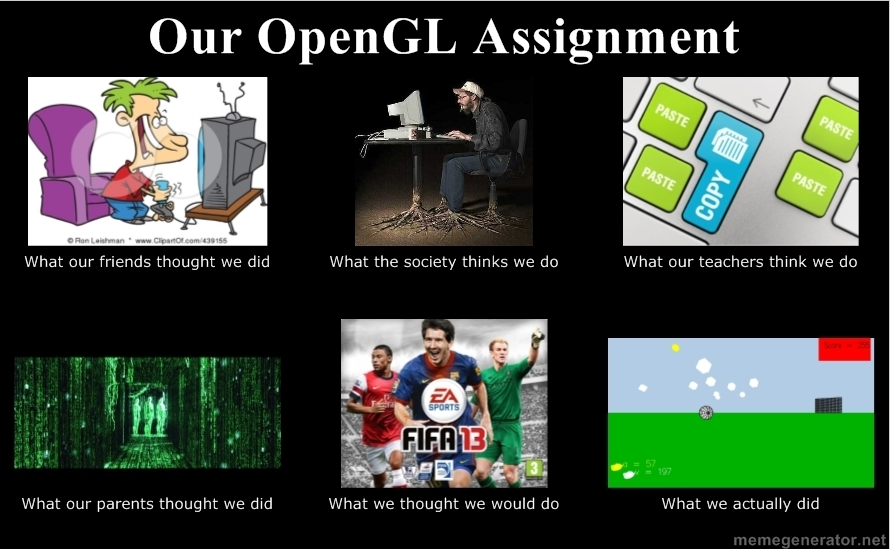
\includegraphics[scale=0.9]{whatwedid.png}\\[1cm]    

% Title
\HRule \\[0.4cm]
{  \huge\bfseries FIFA 2013 in OpenGL }\\[0.4cm]

\HRule \\[1cm]

% Author and supervisor
\begin{minipage}{0.8\textwidth}
\begin{flushleft} \large
\emph{By:}\\
Samir Sheriff [1RV09CS093]\\
Satvik \textsc{N} [1RV09CS095]\\
Vaishakh \textsc{B N} [1RV09CS118]\\

\end{flushleft}
\end{minipage}
\vfill
\date{}
% Bottom of the page
{\large}

\end{center}

\end{titlepage}



\maketitle
\setcounter{secnumdepth}{1}
\section{Introduction}
  Long long ago in a land far away, there lived a camera - a camera that could see using 3D co-ordinates. She had a good friend called Mr. Football. They both had a common enemy called Mr. Goal Post. Using the power of OpenGL, the camera and the football intend to teach the goal post a lesson using matrix transformations. \\
\\Using the power of OpenGL for graphics programming and C++ for object oriented programming (which includes the concepts of data encapsulation, data hiding, inheritance, etc.), we have created a standalone application for a virtual football shootout, inspired by Google’s Olympic Doodle and EA Sports' FIFA series.
Using OpenGL transformations; mouse and keyboard call back functions; lighting transforms; display lists; shading; reflections; anti-aliasing and other OpenGL utilities, we have tried to create an experience that has never been encountered before.\\
\\Classes have been designed to make the game highly flexible and easily extendable to other game applications, using our patented methods of Object-Oriented Design.


\section{Evolution of the System}
The history of our project is an evolutionary
history. Each successive wave of innovation can be seen as a response
either to some limiting aspect of procedural programming preceding it or to
demands from new domains.

To make code management easier, we designed various classes, which we describe below:\\
\begin{enumerate}
\item{\textbf{Coordinates}}\\
Helps in managing 3D coordinates easily, with get and set methods. 

\item{\textbf{RotationAngle}}\\
Helps in managing independent rotations about the 3 axes easily, with get and set methods. 

\item{\textbf{Camera}}\\
If you look at making any game where the scene is larger than can be displayed in the window at once, then you are going to need some type of camera system. It contains methods (that encapsulate trigonometric equations) to:
\begin{itemize}
\item{Move the camera forward and backwards} 
\item{Slide the camera left and right}
\item{Rotate the camera about any of the 3 axes}
\item{Reset the camera to (0, 0, 0)}
\item{Render objects on the screen with respect to the camera's location}
\end{itemize}

\item{\textbf{FootBallField}}\\
Keeps track of all the objects in the world, i.e., 
\begin{itemize}
\item{Sun} 
\item{Sky}
\item{Ground}
\item{Goal Post}
\item{Football}
\item{Scoreboard}
\item{Velocity Initialization Slider}
\item{Projection Angle Initialization Slider}
\end{itemize}

There are only two kinds of objects in this world, my friend:
\begin{itemize}
\item{Those that move along with the camera, and hence, are stationary with respect to the camera - Eg., Sun, Sky, Ground, Scoreboard, Sliders - Display lists are used for these objects.}
\item{Those that do not move along with the camera, and hence, are in motion with respect to the camera - Eg., Football, GoalPost}
\end{itemize}

This class also contains an update method, which automatically calls the respective update methods of the objects in the world to bring about motion with respect to time.

\item{\textbf{Football}}\\
Helps in managing the movement of the football in the Football field. The motion of the ball follows the equations of projectile motion. The following information is tracked:
\begin{itemize}
\item{Coordinates of the ball with respect to (0, 0, 0)}
\item{RotationAngle of the ball with respect to the 3 axes}
\item{Initial Velocity of the ball}
\item{Initial Projection Angle of the ball}
\item{Rates at which the velocity and projection angle change when the ball bounces}
\item{Wind velocity, that causes the ball to sway from left to right, while it moves forward}
\end{itemize}

This class contains methods to:
\begin{itemize}
\item{Set the ball in motion}
\item{Make the ball stationary}
\item{Draw a graphical ball on the screen}
\item{Update the position of the ball as time goes by}
\item{Reset the location of the ball to (0, 0, 0)}
\item{Check when the ball has reached its destination so that the scoreboard can be updated}
\end{itemize}

\item{\textbf{Wind}}\\
Keeps track of wind velocity and wind acceleration, which affects football movement along the x-axis.

\item{\textbf{ScoreBoard}}\\
Keeps track of the number of goals scored by the player, and updates the corresponding graphical display in the top-right corner of the screen. It makes use of our glutStrokeString method. The Scoreboard consists of a red board on top of which the score is engraved for posterity.

\item{\textbf{HorizontalSlider}}\\
Provides a slider interface for the user to select the initial velocity of the ball when the space bar is pressed. It makes use of our glutStrokeString method.

\item{\textbf{VerticalSlider}}\\
Provides a slider interface for the user to select the projection angle of the ball when the space bar is pressed.It makes use of our glutStrokeString method.

\item{\textbf{GraphicString}}\\
This class is used to maintain a pool of characters to be displayed in the intro screen of the game, one at a time, moving in a sinusoidal wave pattern as time goes by. It makes use of our glutStrokeString method.

\item{\textbf{Game}}\\
Contains the main method which initializes the OpenGL State machine with the appropriate variables and methods, starts the main event loop and calls the display and update methods for drawing on the screen.

\end{enumerate}
\section{System Requirements}
Please ensure that the computer on which you plan to run our game, satisfies the following requirements to the T:

\begin{itemize}
\item{Hardware Requirements}:
\begin{itemize}
\item{Processor}: Intel Pentium 4 or above.
\item{RAM}: 2GB
\item{Hard disk}: 200 MB
\item{Appropriate Input and Output Devices}
\end{itemize}
\end{itemize}

\begin{itemize}
\item{Software Requirements}:
\begin{itemize}
\item{Operating System}: Windows 7
\item{IDE}: Visual C++ with OpenGL support.
\item{Latest Graphics card drivers}
\end{itemize}
\end{itemize}
The project has been made open source. The project is hosted in a public repository. To check out the code, head to www.github.com/samiriff/GraphicsAssignments before the world ends.


\section{How to play?}
\begin{enumerate}
\item{Our application can be started either from the Visual C++ IDE by clicking the Run button or by directly opening the application by using the double-clicking feature provided by most modern mice.}

\item{The application opens up in full-screen mode with a resolution of 1920 x 1080, and an animated video is displayed.}

\item{You can either wait for the entire intro to render completely, or, if you're worried that the world is about to end, you can skip it by pressing the 'o' key, which is found on most modern keyboards.}

\item{The game starts off with a sphere, that bears a somewhat strange resemblance to a football, in the center of the screen, with the sky and ground in their appropriate locations as defined by the laws of Nature. A net, which we call a goal post, can be seen in the distance. If you are blessed with a keen eye, you might notice some rotating cubes in mid-air - These are supposed to remotely resemble a visible mass of liquid droplets or frozen crystals made of water or various chemicals suspended in the atmosphere above the surface of a planetary body, which in our case, happens to be the Earth. In layman terms, this mass would be termed a Cloud.}

\item{If you feel the need to view the entire world, feel free to use the camera controls to navigate. The controls are as follows:}
\begin{itemize}
\item{\textbf{a} - Slide to the Left}
\item{\textbf{d} - Slide to the Right}
\item{\textbf{w} - Move forward}
\item{\textbf{s} - Move backward}
\item{\textbf{j} - Rotate about the Y-axis in clockwise direction as seen from above}
\item{\textbf{l} - Rotate about the Y-axis in anti-clockwise direction as seen from above}
\end{itemize}

\item{Once you're done admiring the view and you feel it's time to see some action, use the camera to get the Football within your view. Then use the following controls to set the initial values of the trajectory that the ball will take in the not too distant future:}
\begin{itemize}
\item{\textbf{,} - Toggles the to and fro motion of the  horizontal slider. The current value of this slider is used to set the initial velocity of the football.}
\item{\textbf{.} - Toggles the to and fro motion of the  vertical slider. The current value of this slider is used to set the projection angle of the football.}
\end{itemize}

\item{Once you are perfectly satisfied with the values of the horizontal and vertical sliders, you can give the Space bar a tap on its head, and before you can say "Jack Robinson", lo and behold! The football begins its journey towards the goal post. You can sit back and enjoy the visual treat that our simulation of projectile motion provides.}

\item{Alas! There lurks in the shadows, a mysterious entity - the Wind, which is beyond your power to control. Cross your fingers and hope that the wind doesn't prevent the football from reaching its one and only destination - the goal post. If the football does manage to brave the wind and reach the goal post, you can give yourself a tap on the back when the score on the scoreboard is incremented by one point.}

\item{On the other hand, if the ball doesn't hit the goal post, then today isn't your lucky day. Well, as the old saying goes, \textbf{Try until you succeed} by pressing the \textbf{r} button, found on most keyboards worth their salt, to reset the ball to its original location.}

\item{After you're done, feel free to share our game on sites like ThePirateBay, etc., and if you're in a magnanimous mood today, send your donations to the Code Kshetra Office situated in the dark corners of the universe.}

\end{enumerate}

\section{Motivation}
	Motivation is the psychological feature that arouses an organism to action toward a desired goal and elicits, controls, and sustains certain goal directed behaviors. For instance: An individual has not eaten, he or she feels hungry, and as a response he or she eats and diminishes feelings of hunger. There are many approaches to motivation: physiological, behavioural, cognitive, and social.\\
\\Motivation may be rooted in a basic need to minimize physical pain and maximize pleasure, or it may include specific needs such as eating and resting, or for a desired object. Conceptually, motivation is related to, but distinct from, emotion.
\\ \\ \\


\includegraphics[scale=0.8]{motivation.jpg}\\[1cm]   

\newpage

\begin{thebibliography}{9}

\bibitem{wiki}
  OpenGL Tutorials for Game Development
  \emph{Swiftless Tutorials}
 \url{http://www.swiftless.com/opengltuts.html}

\bibitem{textbook}
Aladeen
\emph{The Official Guide to
Learning OpenGL}
Code Kshetra Inc., Massachusetts,
  10000th Edition,
  2012.


\end{thebibliography}\end{document}
